\chapter{Entwurf}
\label{chapter:entwurf}

In diesem Kapitel werden die Anforderungen der Modelle erläutert und die Herangehensweise im Konzept beschrieben.

\section{Anforderungen}

%Anforderungsanalyse 

% Funktionale: 
% blatt nicht erkennen, sondern direkt die Krankheit, Visualisieren
%- Blattkrankheiten, hier benennen 
%- Erkennung von 4 Krankheiten und gesunde blätter
%-- zwei verschiedene Ansätze: Custom Modell, Transfer LEarning
%- speziell ein Voter entwerfen -> für blights
%-- ähnlich symptome aber sehr schwierig zu unterscheiden sind
%- Visualisierung der Schichten


In dieser Masterarbeit soll das zu erstellende Modell, welches mithilfe von Faltungsnetzen realisiert werden soll, die Erkennung der vier Krankheiten sowie gesunden Blättern von einem vorgegebenen Datensatz ermöglichen. Die Krankheiten, hier Dürrfleckenkrankheit, Tomato Yellow Leaf Curl Virus, Samtfleckenkrankheit und Krautfäule, unterscheiden sich ausgehend in der Ausprägung der Symptome stark. Die zwei Krankheiten, Krautfäule und Dürrfleckenkrankheit, weisen vergleichbare Symptome auf. Deswegen sollen mehrere Modelle erstellt werden, die mit einem Voter verbunden sind. Dieser Voter soll aus den Ergebnissen der verschiedenen trainierten Modelle die passende Ausprägung bestimmen. 

Da neuronale Netze wie eine Black-Box wirken, sollen die Aktivierungen der Schichten visualisiert werden, um Merkmale in der entsprechenden Schicht zu verdeutlichen.

\section{Konzept \& Entwurf}

Im Konzept werden die verschiedenen Ansätze erläutert, wie die Modelle aussehen sowie erstellt werden könnten. Hier wird die Herangehensweise eines typischen Faltungsnetzes beschrieben. Des Weiteren wird auch ein anderer Ansatz gezeigt, wie ein Faltungsnetz mithilfe von vortrainierten Modellen erstellt werden kann. Außerdem wird auch ein Voter vorgestellt, um bessere Ergebnisse in der Klassifikation erzielen zu können. All diese Ansätze werden mittels einer Bibliothek implementiert, die in diesem Abschnitt bei einem Vergleich ausgewählt wurde.

\subsection{Wahl der Bibliothek}
%Nicht funktionale:
%- Welche Bibliothek? Vergleich der Bibs?
%--Performance also auf Grafikkarten, Prozessoren,  oder Architektur, die das ermöglichen,


In den Abschnitten \ref{sec:keras} und \ref{sec:pytorch} wurden zwei unterschiedliche Bibliotheken vorgestellt, die die Erstellung von neuronalen Netzen ermöglichen. Dennoch ist noch zu klären, welche der Bibliotheken optimal für die Erstellung eines Faltungsnetzes ist. Deswegen werden sie unter bestimmten Kriterien analysiert. Die genaue Beschreibung der Kriterien wird hier aufgeführt:

\begin{itemize}
	\item Die einfache Einarbeitung:
	
	Hierbei wird die Frage geklärt, ob sehr viel Detailwissen von neuronalen Netzen für die Anwendung vorausgesetzt wird und wie tief das Wissen über die Implementierung mittels eigener Implementierung sein muss.
	
	\item GPU-Support:
	
	Hier ist es interessant zu wissen, ob die Möglichkeit besteht, eine Grafikkarte für das Training der Modelle anwenden zu können. Des Weiteren wird hier untersucht, ob die Einbindung der Grafikkarte schwierig und aufwändig ist.
	
	\item Programmierfreundlichkeit:

	Unter dem Kriterium Programmierfreundlichkeit fällt alles bezüglich der Erstellung der Modelle. Außerdem wird hier untersucht, ob das Starten des Trainings aufwendig und die Benutzung eines Debuggers möglich ist. 
	
	\item Zeitaufwand:
	
	Der Zeitaufwand für die Erstellung und das Training der Modelle sollte gering sein.
	 
	\item Funktionalitäten:
	
	Ein weiterer Aspekt ist der Umfang der Funktionalität. Hier wird untersucht, ob dieser groß genug ist, um komplexe Architekturen zu ermöglichen.
	
\end{itemize}

Bei der Erstellung von neuronalen Netzen unterscheiden sich diese beiden Bibliotheken stark. In PyTorch werden die neuronalen Netze wie Klassen definiert, die ein Modul aus der Torch-Bibliothek erweitern muss. Mit bereitgestellten Schichten wird das Modell erweitert. Im Konstuktor werden die Eingabe- und Ausgabegrößen definiert, die in der \textit{forward()}-Methode der Klasse ausgeführt werden. Der große Vorteil von PyTorch ist, dass alle Klassenmerkmale von Python genutzt werden können, um die Definition von neuronalen Netzen übersichtlicher zu gestalten. Die Bibliothek Keras kann das neuronale Netze mittels der \textbf{Functional}-API als eine Reihe von Funktionsaufrufen, die nacheinander ausgeführt werden und in sequentieller Reihenfolge vorliegen. Dabei entspricht die Ausgabe der ersten Schicht der Eingabe der zweiten Schicht. Insgesamt lassen sich mit Keras viel schneller Modelle definieren, da das Wissen bezüglich der objektorientierten Programmierung nicht benötigt wird. 

Außerdem verbirgt Keras alle Implementierungsdetails, so dass die Definition von Schichten intuitiv bleibt. Meistens reicht die Standardvorlage aus. Die Problematik an solchen Vorlagen liegt darin, dass komplexe Architekturen nicht gegeben sind und somit selbst implementiert werden muss. Diese Implementierung erfolgt auf der untersten Ebene. Das heißt, dass alle Matrix-Operationen korrekt sein müssen. Des Weiteren gibt es keine Möglichkeiten, die Ausgaben der neu definierten Schicht auszugeben. PyTorch verlangt von dem Benutzer die Angabe bezüglich der Eingabe und Ausgabe jeweiliger Schichten. Da der Berechnungsgraphen in PyTorch dynamisch ist, ist es möglich, zur Laufzeit die Werte auszugeben. Weiterhin ist der Wechsel zwischen Tensoren und Numpy Arrays in PyTorch mithilfe von zwei Operationen einfacher gelöst. 

Das Trainieren des Modells ist in Keras mit einer einzelnen Zeile Code gelöst. Hierbei wird die \textit{fit()}-Methode mit den nötigen Parametern aufgerufen. In PyTorch muss das Training implementiert werden. Folgende Schritte sind hierbei nötig: Gradienten müssen bei jedem Start eines Batches initialisiert werden. Mit dem passenden Modus werden die Daten nach vorne propagiert. Anschließend werden die Daten wieder zurückpropagiert, um den Verlust berechnen und die Gewichte aktualisieren zu können. 

Wenn das passende Backend, zum Beispiel TensorFlow für GPU, installiert wurde, dann erkennt Keras automatisch die Grafikkarte und diese wird als Standardkonfiguration gesetzt. Die PyTorch-Bibliothek hat diese automatische Erkennung von Grafikkarten nicht. Jede Variable, Modelle und Daten müssen daher auf die Grafikkarte übermittelt werden. 

In der Tabelle \ref{bib_comp} werden die Bibliotheken mithilfe von drei Sternen bewertet. Hierbei zeigt sich Keras als geeignete Bibliothek. Deswegen wird Keras für die Implementierung in dieser Masterarbeit verwendet.
~\newline
%% hier kommt eine Tabelle
\begin{figure}[h]
\center
\begin{tabular}{|c|c|c|}
	\hline
	Kriterien/Bibliotheken & Keras & PyTorch \\
	\hline
	Einfache Einarbeitung & *** & ** \\
	\hline
	GPU-Support  & *** & ** \\
	\hline
	Programmierfreundlichkeit  & ** & ** \\
	\hline
	Zeitaufwand  & *** & ** \\
	\hline
	Funktionalitäten  & ** & *** \\
	\hline
\end{tabular}
\caption{Ein Vergleich zwischen den Bibliotheken Keras und PyTorch.}
\label{bib_comp}
\end{figure}



\newpage
\subsection{5-Klassen Modell}

Der Ansatz erfolgt nach dem typischen Aufbau von tiefen Faltungsnetzen. Paare, die aus Faltungs- und Poolingschichten bestehen, sind die Bausteine des Modells. Diese werden oft wiederholt, um ein tiefes Netzwerk zu erhalten. Zwischen den Paaren können Dropout-Schichten auftreten. Mit dieser Struktur sollte das Faltungsnetz Merkmale automatisch aus den Bildern extrahieren können.

\subsection{Modell mittels Transfer Learning}
Eine weitere Möglichkeit die Klassifikation der fünf Klassen zu ermöglichen, ist die Nutzung von vortrainierten Modellen. Der Vorteil von vortrainierten Modellen ist, dass solche Modelle sehr große Datensätze mit mehreren hundert Klassen trainiert wurden. Dadurch können die Faltungsschichten in den unteren Ebenen grundlegende Merkmale, die die Ausprägungen der Symptome eventuell gelernt haben, nutzen, um die vier Krankheiten klassifizieren zu können. Dabei werden die Gewichte des vortrainierten Modells eingefroren, so dass das zu erstellende Modell diese nutzen kann.  
Bekannte vortrainierte Modellen sind beispielsweise VGG16, VGG19, DenseNet und ResNet. 


\subsection{Voter}


Neuronale Netze können nicht immer korrekt die Klasse bestimmen. Je nachdem wie das Modell trainiert ist, kann eine Klasse oft falsch klassifiziert werden. Zum Beispiel erkennt ein Modell die Dürrfleckenkrankheit als gesunde Blätter an. Um eine gewisse Sicherheit zu erlangen, kann das Eingangsbild bei anderen Modellen, die unterschiedliche Architekturen haben, getestet werden. Hierdurch lässt sich herausfinden, ob die Dürrfleckenkrankheit korrekt erkannt wurde. Auf dieser Basis kann ein Mehrheitsvotum mit drei Modellen stattfinden, um die Fehlerrate zu reduzieren. Hierbei kann die häufigste genannte Klasse unter den drei Modellen als korrekte Klasse angesehen werden.


Die Abbildung \ref{voter_image_funel} veranschaulicht die Idee eines Voters. Drei Modelle versuchen das Eingangsbild zu klassifizieren. Die Ergebnisse werden dem Voter übertragen und dieser klassifiziert endgültig die Klasse \glqq Healthy\grqq.


\begin{figure}[h!]
	\centering
	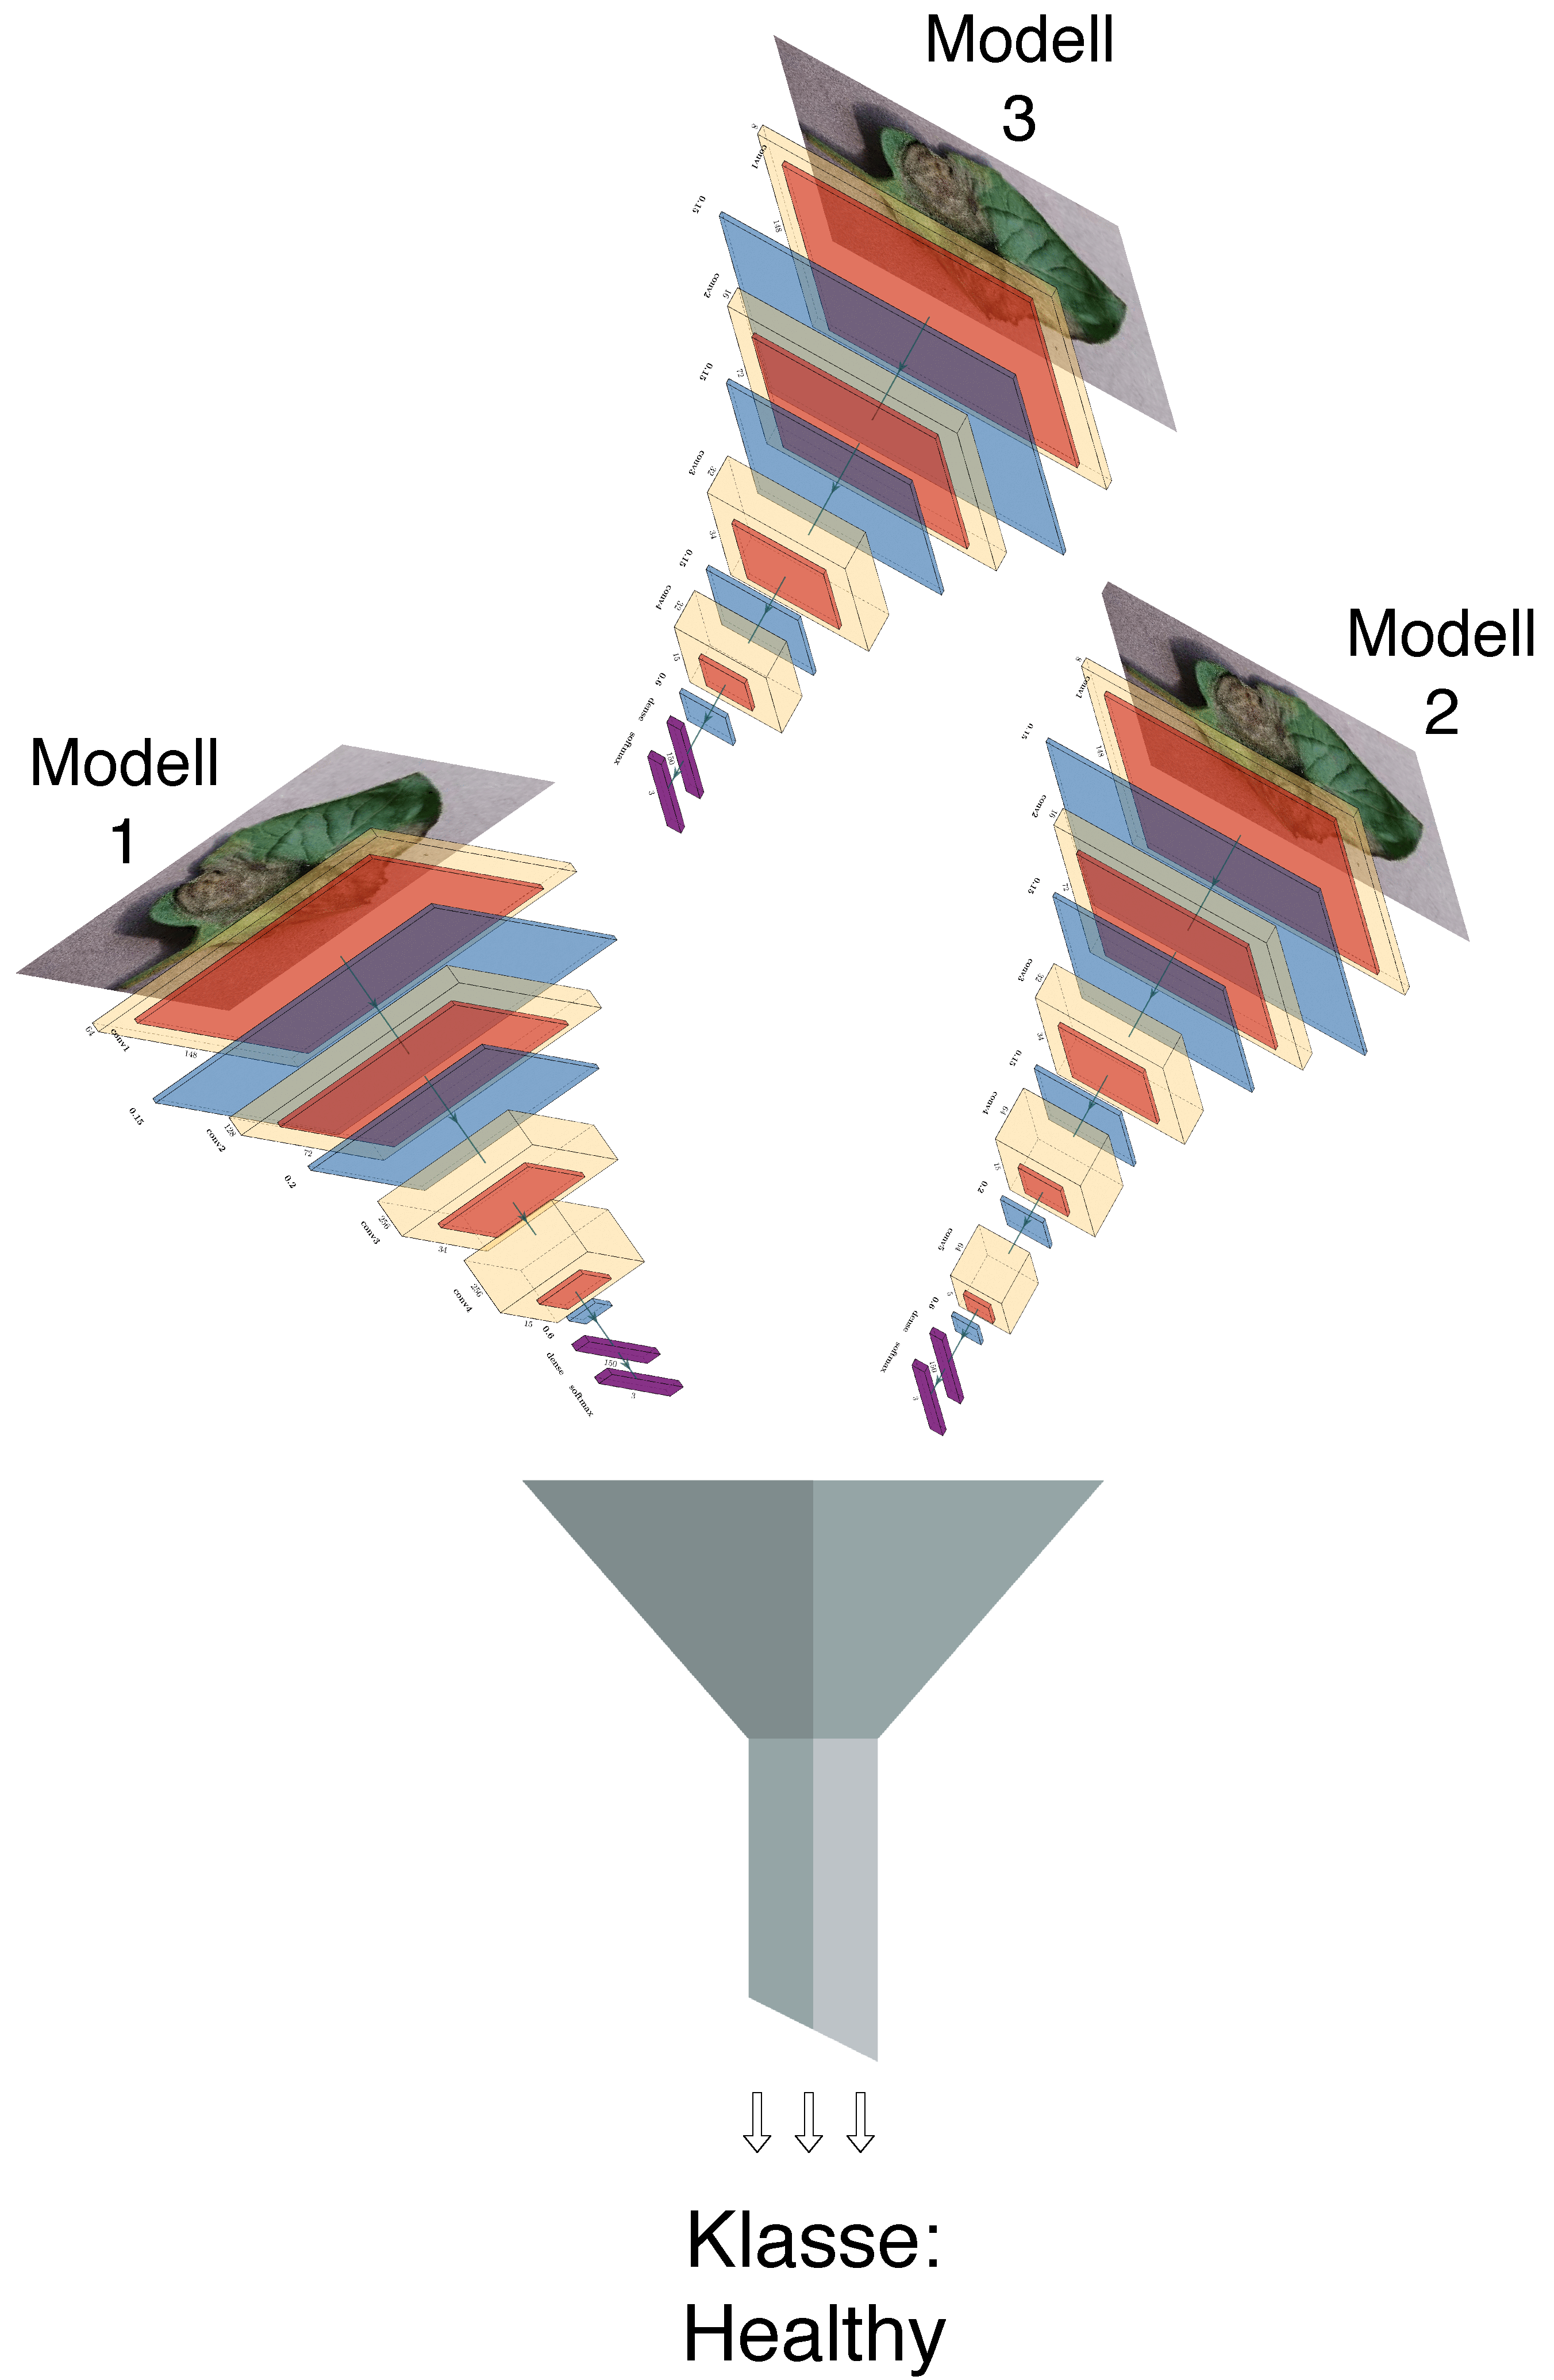
\includegraphics[width=\textwidth]{bilder/voter_image_funel.pdf}
	\caption{Darstellung eines Voters mit drei Modellen. Der Voter hat aus den Ergebnissen die Klasse \glqq Healthy\grqq~bestimmt (eigene Darstellung).}
	\label{voter_image_funel}
\end{figure}


